%# -*- coding: utf-8-unix -*-
% !TEX program = xelatex
% !TEX root = ../thesis.tex
% !TEX encoding = UTF-8 Unicode
%%==================================================
%% chapter01.tex for SJTU Master Thesis
%%==================================================

%\bibliographystyle{sjtu2}%[此处用于每章都生产参考文献]

\chapter{Introduction}
\label{sec:intro}
Nowadays, recommender systems have been widely used in most Internet-based services, such as news feeds \cite{wang2017dynamic,liu2010personalized} and e-commerce platform \cite{rendle2010factorizing}.
The goal of recommender system is to select the items or contents that the target user tends to like, which alleviates the information overload in a large margin \cite{zhang2017deep} of online information systems.

The researchers in both academic and industrial fields have devoted many efforts on this research hotspot.
Among the existing methods, the most widely adopted solution is based on collaborative filtering originating from \cite{goldberg1992using}.
It achieves the goal of recommendation through learning only from historical user-item interactions, either explicit (i.e., user ratings over items) or implicit (i.e., user clicks) feedbacks \cite{zhang2017deep} without exogenous information about items or users.
The collaborative filtering (CF) methodologies seek to capture the collaborative relations among different users with similar tastes \cite{koren2008factorization} to provide recommendations to the target user.

% spatial information: user-item interactions
%\kan{need an illustration of user-item interaction graph to represent first-order interactions of the target item and the target user.}
\begin{figure}[h]
	\centering
	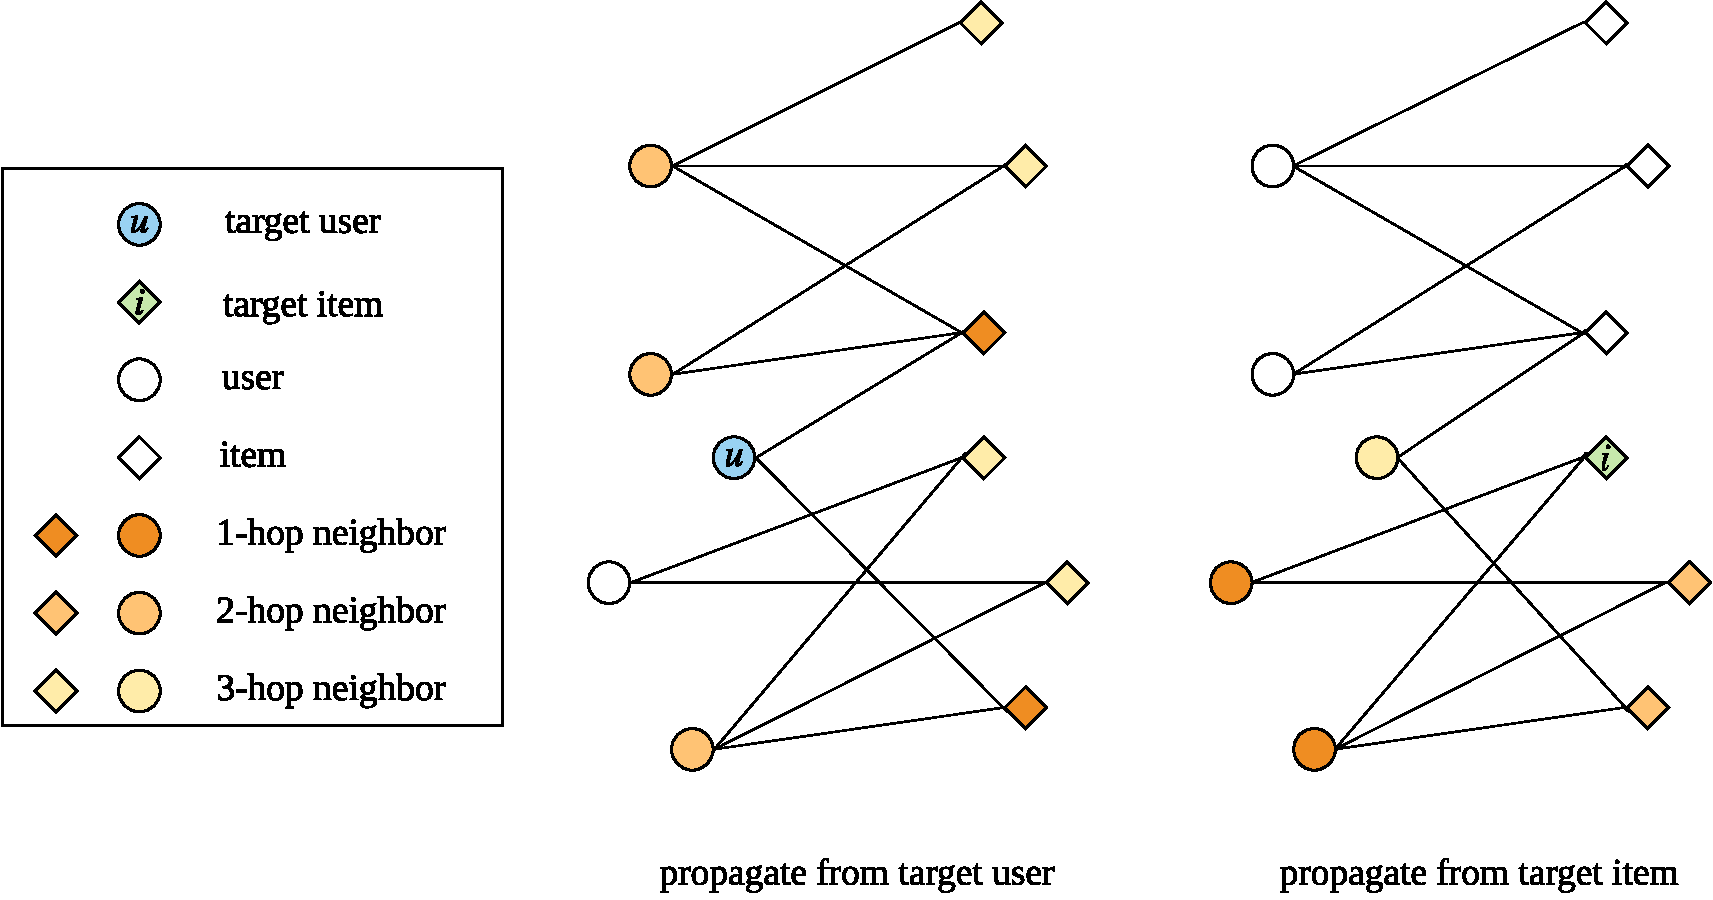
\includegraphics[width=1.0\columnwidth]{intro.pdf}
	\caption{Graph illustration of target user/item-rooted subgraph.}
	\label{fig:bi-graph}
\end{figure}
% Some methods \cite{niu2018collaborative,talasu2017link,ying2018graph,fadel2018link,van2017graph,wu2019session} regard the recommendation task as a link prediction problem with the consideration of the existing node connections (user-item interactions), as is shown in Figure~\ref{fig:bi-graph}.
% The view of traditional collaborative filtering is a first-order graph pattern mining since the interactions between the target user and the visited items conduct the first-order connections from the user in the bipartite graph of user-item interactions.
% Nevertheless, these methodologies only regard the feature extraction for the target user (or the target item) as neighborhood gathering \cite{kipf2016semi}, which does not incorporate the collaborative influence among the gathered nodes \kan{to refine; to add collaborative relations.}, as shown by the dotted line in Figure~\ref{fig:bi-graph}. \jiarui{refine figure 1 or sentence}
% Moreover, they consider the related interactions in the bipartite graph to the target, while ignoring the temporal patterns for the evolving graph of user-item interactions.
Some methods \cite{niu2018collaborative,talasu2017link,ying2018graph,fadel2018link,van2017graph,wu2019session} regard the recommendation task as a link prediction problem, which is to predict the probability of link relation, e.g., clicks and conversions, between the target user and the target item.
They consider the existing node connections (user-item interactions) as the feature for link prediction.
The view of traditional CF is a first-order graph pattern mining since the interactions between the target user and the visited items conduct the first-order connections in the user-item bipartite graph as is shown in Fig.~\ref{fig:bi-graph}. 
%\kan{it seems that kth-order means ``to predict k links'', but we only use k links as features. it should needs confirmation.}
These methodologies only use the first-order neighbors through one-hop propagation to represent the target user (or target item) and learn the representations of users/items though reconstructing the rating matrix.
These models utilize the "collaborative" information in an implicit way by learning the representation of users and items. However, they ignore the collaborative information that can be found by propagating over the user-item bipartite graph.
That is to find the users who share the same interests  (interacted with same group of items) with the target user.
These users from this subgraph can be used to enhance the representation of the target user. And it can be done in a similar way from the side of the target item. The propagation process over the subgraph can be conducted many times as shown in Fig~\ref{fig:bi-graph}.

% another con is the ignorance of collaborative relations

% temporal dynamics 
As has been stated in many related works \cite{hidasi2017recurrent,koren2009collaborative,he2016vista,agarwal2009spatio}, the temporal dynamics have high impacts on future user behaviors, especially accounted for concept drifting \cite{widmer1996learning}, long-term behavior dependency \cite{koren2009collaborative}, periodic patterns \cite{ren2018repeatnet}, etc.
However, most CF models regard the user-item bipartite graph as a static entirety while ignoring the temporal dynamics of user-item interactions.
Yet some other researchers tend to utilize state-based methods \cite{he2016fusing,he2016vista} or sequential modeling \cite{hidasi2017recurrent,tang2018personalized,ren2019lifelong} to capture the dynamic user behavior patterns, especially for sequential recommendation \cite{huang2018improving,chen2018sequential,kang2018self,tang2018personalized} problem.
There are two drawbacks hidden in the existing sequential modeling works.
The one is that they only consider the changing preference of the user, while the temporal dynamics of the item have been abandoned.
For example, the popularity of the existing item may change over time \cite{koren2009collaborative} according to some factors such as gloves are more popular in winter than in summer; and some products may involve sales promotion in some time to attract new group of users. %Such that people may show preference to different items at different time even though their tastes remain the same during that period.
%The other con is that few of them utilize the spatial information of the graph for the sequential modeling at each time, thus lacking of global pattern mining.
Such that the same item may attract different users at different time even though its properties are stable along the time.
The other con is that few of them utilize the collaborative information provided by similar users or similar items. These sequential recommendation models tend to only memorize the target user's own interest dynamics while they lack of a wider range of considerations.
% collaborative filtering and sequential recommendation
% drawbacks


Generally speaking, the \textit{spatial} collaborative graph information and the \textit{temporal} sequential patterns both influence the final recommendation.
To comprehensively utilize the spatial-temporal information with collaborative filtering, we propose \textbf{S}equential \textbf{Co}llaborative \textbf{Re}commender (\score).
The model firstly conducts the incremental subgraphs originating from the target user and the target item along time.
Secondly, it fully utilizes the spatial information given by the local subgraph through mining the collaborative patterns with multi-hop propagation over graph neighbors.
%by mining the patterns through multiple hop propagation over graph 
Finally, it also captures the sequential patterns along the evolving user-item graph from both sides of the target user and the target item.%and finally adopts collaborative filtering for the subgraphs at each time slice for better modeling the evolving graph patterns of user (item) similarities.

Specifically, for user-item interaction graph at each time slice, we utilize the proposed \textit{Co-Attention Graph Network} to aggregate the spatial information gathered by multi-hop propagation in a collaborative manner.
Then we apply a non-linear recurrent neural network (RNN) for modeling the temporal patterns of the evolving graph, with the consideration of the obtained collaborative relations.
By this way, our model has the knowledge of (i) which group of people would share the similar tastes at each time (through multi-hop propagation on the graph), (ii) how their preferences evolve along the timeline (through non-linear recurrent model).
Moreover, not just modeling the user behaviors, \score~ can also consider from the item side and well capture the item trends for better user-item matching in the final recommendation by utilizing an interactive attention mechanism.
For example, this recommender system may present Christmas card to a user when the holiday is coming even \textit{before} her interacting with any related items. This goal would be obtained by using the interests of similar users to her and model the temporal dynamics properly.

% advantage
% a new perspective for recommender system with spatial-temporal pattern mining
% non-linear temporal pattern mining and collaborative relation discovery through co-attention mechanism
% dynamic system for varying user preferences and diversified trends of items
To the best of our knowledge, this is the first work which models the sequential recommendation task as incremental graph learning problem. It applies unified spatial-temporal graph pattern mining with collaborative filtering for the recommender systems.
The contribution of the paper lies in three-fold:
\begin{itemize}[leftmargin=5mm]
	\item \textbf{Spatial and Temporal Graph Pattern Mining.} We slice the user-item interactions as a series of evolving bipartite graph along the timeline, and propose a comprehensive framework with spatial-temporal pattern mining for final recommendation.
	\item \textbf{Dual Sequence Modeling.} We apply the spatial and temporal pattern mining from both sides of user and item, which derives a comprehensive modeling result.
%	 \textit{Co-Attention Graph Network} to aggregate multiple hops information on the user-item interaction graph in a collaborative manner.
%	\item \textbf{Temporal Graph Pattern Mining}: We propose \textit{Interactive Attention Mechanism} to model the problem of link prediction (between the target user and target item) for the dynamic incremental graphs. We use subgraph sequences from both target user's and target item's side.
	\item \textbf{State-of-the-art Performance.} We evaluate and compare our model with several strong baselines over three real-world and large-scale recommendation datasets. The results have proven the efficacy of \score ~model.
\end{itemize}

The rest of the paper is scheduled as below.
In Section~\ref{sec:rel}, we discuss about some related works.
Section~\ref{sec:method} presents the \score~model in detail and we also make some discussion about the relatedness to the existing works.
We conduct some comprehensive experiments and present the experimental setups with the corresponding results in Section~\ref{sec:exps}.
Finally we conclude the paper and point out some future works in Section~\ref{sec:con}.
